\section{Classification of indefinite unimodular forms} 
Today we will discuss the proof of Hasse-Minkowski, even forms, and the $E_8$ lattice. Let us restate the Hasse-Minkowski theorem.
\begin{namedthm}{Hasse-Minkowski Theorem} 
    An indefinite unimodular form is determined up to isomorphism by its rank, signature, and type (even or odd). 
\end{namedthm}
\begin{example}
    An odd indefinite unimodular form is isomorphic to $p I_+ \oplus qI_-$
\end{example}
Some comments on the proof: the proof hingers on finding an \emph{isotropic} vector $x\neq 0$, i.e. $x\cdot x=0$. Over $\R$, indefiniteness is equivalent to the existence of an isotropic vector. Over $\Z$, it suffices to find $x$ over $\Q$, from then we can scale it up to lie in $\Z$.

There is a big idea in number thoery which deals with thinking about \emph{local} and \emph{global} principles. We have $(\Lambda, \sigma)$ an indefinite unimodular form. Then considering  $\Lambda \otimes \Q$, over $\Q$ the quadratic form $x \mapsto  x \cdot x$ is diagonalizable; \[
    x=(x_1,\cdots ,x_r) \mapsto  a_1x_1^2+\cdots +a_r x_r^2 =q(x) \quad \text{for } 0\neq a_i  \in  \Q.
\] We want to solve $q(x)=0$; this is what we did in high school adding a few numbers and the condition that the solution must be rational. ``Global'' solutions over $\Q$ give rise to ``local'' solutions over the ``places'' (completion) of $\Q$. An isotropic vector  over $\Q$ gives rise to an isotropic vector over $\R$, and isotropic vectors over the $p$-adics $\Q_p$ for $p$ a prime. So solutions over $\Q_p$ are roughly equivalent to a sequence of vectors $x(n) \in  \Lambda$ such that $q(x(n))\equiv 0 \pmod {p^n} $, such that $x(n)$ refines $x(n-1)$.

\subsection{The Hasse-Minkowski local-to-global principle}

The Hasse-Minkowski local to global principle says that for quadratic forms $q$, existence of local isotropic vectors for all $p$ over $\R$ implies existence of a global isotropic vector. This works best in this area of number theory; if we move to elliptic curves there are examples a plenty of local objects that don't translate globally. See Serre's \emph{A Course in Arithmetic} for a reference for all of this.

It turns out that over $\Q_p$, quadratic forms in $\geq 5$ variables \emph{always} have an isotropic vector for all $p$ over $\R$. In fewer variables ($\leq 4$), being indefinite and unimodular implies that a $p$-adic isotropic vector exists. Over the reals, indefiniteness gives rise to an isotropic vector.
How does this help? Say $\Lambda$ is odd, indefinite, and unimodular. Find $0\neq x \in \Lambda$, $x\cdot x=0$.
\begin{namedthing}{Check} 
   It is not trivial but not too complicated either to check that $x=me+nf$, where $e\cdot e=1, f\cdot f-1$, $e \cdot f=0$ for some $m,n \in \Z$. In other words, $x$ lies in a copy of $I_+\oplus I_-$.
\end{namedthing}
Since we are working with quadratic forms, we must do what every proof in quadratic forms does, which is proceed by induction on the rank. Now $\Lambda=(I_+ \oplus I_-) \oplus _{\text{orthog} }\Lambda'$, so either $\Lambda'\oplus I_+$ or $\Lambda' \oplus I_-$ is indefinite. From here induct on the rank.

\begin{cor}[Odd case of H-M]
    For all unimodular forms $\Lambda ,$ if $c \in \Lambda$ is a characteristic vector ($c *x \equiv x \cdot x \pmod 2$ for all $x$), then $c \cdot  c \equiv \tau(\Lambda) \pmod 8$.
\end{cor}
\begin{example}
    If $\Lambda$ is even, then $\tau(\Lambda) \in  8 \Z$. 
\end{example}
\begin{proof}
    Stabilizing $\Lambda$ by adding a copy of $I_+$ or $I_-$ adds  $\pm 1$ to $\tau$, $\pm 1$ to $c \cdot c$. So we reduce to the case of being odd or indefinite, so this leads to $pI_+ \oplus qI_-,\tau = p-q$, $c=(1,\cdots ,1)$. Note that $ c \cdot  c =p-q$, and the fact that this particular characteristic vector has square \emph{equal} to the signature implies that \emph{any} characteristic vector is congruent to the signature$\pmod 8$.
\end{proof}
\subsection{The even case}
The proof for Hasse-Minkowski for \emph{even} unimodular forms is an intricate reduction to the \emph{odd} case. The two basic even unimodular forms $U,\Z^2$, $\left[ \begin{smallmatrix}
    0 & 1 \\ 1 & 0
\end{smallmatrix}\right] $ is an even pairing over $\Z \oplus \Z^k$. The other is $\boxed{E_8}$, which is positive definite of rank 8. Then $U \cong -U$, and $-E_8$ is negative definite. So every even unimodular form is isomorphic to $rU \oplus s(\pm E_8)$ for some non-negative integers $r,s$.
\begin{example}
    It turns out that if $\Q \subseteq \C \mathrm{P^3}$ is a smooth quartic surface, then $b_2(Q)=22, \tau(Q)=-16$, and has even type. Then by H-M we get that this indefinite form is isomorphic to $3U \oplus 2(-E_8)$.
\end{example}
\subsection{The $E_8$ lattice}
Let us start by defining the $D_8$ lattice. Define \[
D_n  := \left\{x \in \Z^n  \,\big|\, \sum x_i  \in 2\Z\right\}  \subseteq \Z^n \subseteq \R^n .
\] In two dimensions, $D_2$ consists of squares around the origin. Let $\gamma = \frac{1}{2}(e_1 + \cdots + e_8) \in \R^8.$ Set $E_8 = D_8+(\gamma +D_8) \subseteq \R^8$ with $\cdot $ being the dot product. We can check that this takes integer values. We could also say that \[
E_8= \left\{ x \in \Z^8 \cup  \left(\Z + \frac{1}{2}\right)^8 \,\Big|\, \sum x_i  \in 2\Z\right\} .
\] This is an even lattice; if $x \in E_8$, then $x \cdot x=\sum x_i  ^2 \equiv \sum x_i \equiv 0\pmod 2$. There is a basis $(v_1,\cdots ,v_8)$, where $v_i =e_{i+1}-e_i $ for $i \leq i \leq 6$, $v_7=\frac{1}{2}(e_1+e_8)- \frac{1}{2}(e_2 + \cdots +e_7)$, and $v_8= e_1+e_2$. The $v_i $'s are all \emph{roots}, i.e. vectors of square two, or $v_i  \cdot v_i =2$. For $i\neq j$, $v_i \cdot v_j $ is usually zero, but there are some exceptions. We have  $v_i  \cdot  v_{i+1}= -1$ for $1 \leq i \leq 5$, $v_7 \cdot  v_1 = -1, $ and $v_8 \cdot  v_2=-1$.  A more memorable way of encoding this diagram is by the Dynken diagram, where nodes are basis vectors and edges are vectors $v_i,v_j $ such that $v_i  \cdot v_j =-1$.
{\color{red}todo:figure} 
\begin{figure}[H]
\centering
 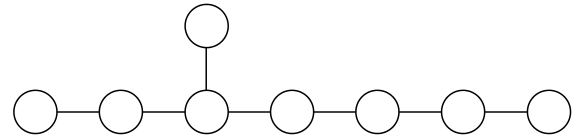
\includegraphics[width=0.6\linewidth]{figures/e8.png}
 \caption{The Dynkin diagram of $E_8$.} 
 \label{e8} 
\end{figure}

To see that $E_8$ is unimodular, we have $\Lambda \supset \Lambda'$ a sublattice with $\det \Lambda' = [\Lambda : \Lambda'] \det \Lambda$. Both $\Z_8$ and $E_8$ contain $D_2$ as an index 2 sublattice, which implies that $\det E_8= \frac{2}{2}\det \Z^8 =1$.

